% glcd-sd.tex
% This is the project document.

\documentclass[11pt,a4paper]{article}

\usepackage{graphicx}
\usepackage{indentfirst}
\usepackage{verbatim}
%\usepackage{multirow}
%\usepackage{fancybox}
%\usepackage{endnotes}

\title{Graphic LCD Library: ATmega16, SD Card and SED1520}
\author{sun\_ge@yahoo.cn}

\begin{document}

\maketitle

\section{Project Origin}
I bought a SED1520 based 122x32 dots graphic LCD, in order to display graphic and
Chinese character. But the GB2312 coded font file(there are more than six thousands
16x16 dots Chinese characters in it) is too large(267616 Bytes) to fit the AVR's internal flash
memory. So I decided to store this font in SD card.\\
In this project, I provide:
\begin{enumerate}
\item A library to access SD/MMC card using SPI;
\item A library to display 5x7 ascii characters, 16x16 Chinese characters, and xbm grahpics
on SED1520 based 122x32 LCD.
\end{enumerate}

\section{Hardware}

A drawing and some ascii characters was displayed. The 5x7 ascii font and drawing
was stored in ATmega16's flash. For hardware connection, please see glcd.h.\\
\begin{center}
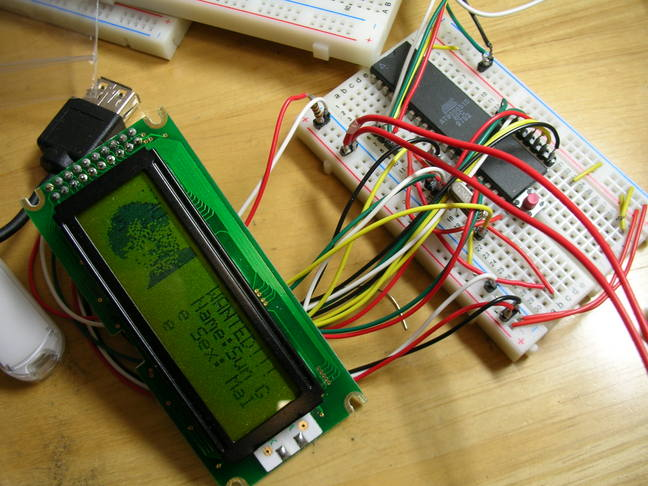
\includegraphics[scale=0.9]{glcd-sd-1.jpg}
\end{center}

Some Chinese characters was displayed. The 16x16 GB2312 font (267616 Bytes)
was stored in a 8MB SD card.(It's stored in raw data, without file system support).\\
For hardware connection, please see glcd.h and mmc.h.\\
\begin{center}
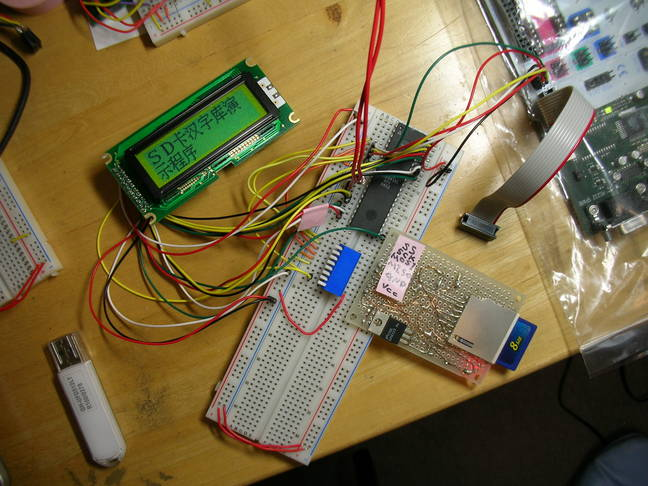
\includegraphics[scale=0.9]{glcd-sd-2.jpg}
\end{center}

SD card need a 3.3V VCC, since ATmega16 was powered by 5.0V, a 5V to 3.3V level
converter is necessary between signal pins.\\
\begin{center}
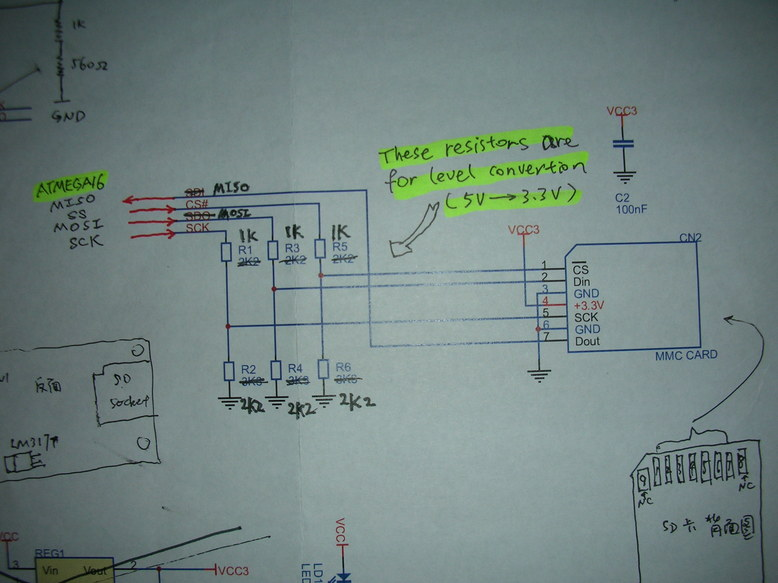
\includegraphics[scale=0.9]{sd.jpg}
\end{center}

\section{Source Code}
Source contains: font5x7.h, mmc.h, mmc.c, glcd.h, glcd.c, hz-xbm.h, pic1.xbm, q.xbm, main.c 
and Makefile.\\
The 16x16 GB2312 font file can be found in package \textit{zhcon} of Fedora Core 3 Linux system,
with the name \textit{hzk16.bpsf}. 

Sources can be compiled and installed by AVR GNU Tools Chain.

\subsection{ASCII Font Header: font5x7.h}
\verbatiminput{font5x7.h}

\subsection{MMC/SD Library Header: mmc.h}
\verbatiminput{mmc.h}

\subsection{MMC/SD Library: mmc.c}
\verbatiminput{mmc.c}

\subsection{Graphic LCD Library Header: glcd.h}
\verbatiminput{glcd.h}

\subsection{Graphic LCD Library: glcd.c}
\verbatiminput{glcd.c}

\subsection{Demo Program: hz-xbm.h, pic1.xbm, q.xbm, and main.c}
\emph{ATTENTION: main.c must be in GB2312 encoding due to display Chinese characters!}\\
hz-xbm.h:\\
\verbatiminput{hz-xbm.h}

pic1.xbm:\\
\verbatiminput{pic1.xbm}

q.xbm:\\
\verbatiminput{q.xbm}

main.c:\\
\verbatiminput{main.c}

\subsection{Makefile}
\verbatiminput{Makefile}

\end{document}
%%% Local Variables:
%%% coding: UTF-8
%%% mode: latex
%%% End:
